\documentclass[13pt]{beamer}
\mode<beamer>{%
  \usetheme[]{CambridgeUS}}
\usepackage{lmodern, amssymb,amsmath, graphicx, hyperref}
\usepackage[normalem]{ulem}
\usepackage{csquotes}
\usepackage{appendixnumberbeamer}
\graphicspath{{Figs/}}


 \title{Campaign Contributions and Bureaucratic Oversight:} 
 \subtitle{A Case Study of the Federal Energy Regulatory Commission}
    \author[Judge-Lord, Grimmer, Powell]{Eleanor Neff Powell \\ Booth Fowler Associate Professor \\ University of Wisconsin-Madison}
    \date[\today]{Joint with Devin Judge-Lord\thanks{Ph.D. Candidate, University of Wisconsin-Madison} and Justin Grimmer\thanks{Professor, Stanford University} \\ \bigskip \today}
\begin{document}
\begin{frame}
\maketitle
\end{frame}

% Hi, My name is Devin Judge-Lord
% I am presenting work with coauthors Justin Grimmer and Ellie Powell based on a very large new database of letters and emails written by members of Congress to federal agencies. We have spent the past 2 years collecting and coding these data, and I am excited to share the very first results from this project. 

% We started with a common intuition that Members of Congress have limited time and attention to divide among, for example, constituency work and policy work. We have come to question the value of this intuition for explaining  at least this aspect of legislator behavior.
% We did not find a tradeoff between being attentive to constituents and influential in washingon; instead, by our measure, some legislators are both and some are neither.

% I am going to introduce our data and show that, in fact, the same members who do more policy work also do more constituency service and that both seem to be connected to institutional power. 

% But first, I want to talk a little bit about our definitions and intuitions about constituency service.

% From where did our, possibly incorrect intuition arise? [SLIDE]

%%%%%%%%%%%%%%%%%%%%%%%%%%%%%%
\begin{frame} 
\frametitle{Arnold's Impact: Studying Congress-Bureaucracy}
\Large

\begin{itemize}
\item Arnold's classic book \emph{Congress and the Bureaucracy: A Theory of Influence}
\begin{itemize}
\item[-]  Theory of bureaucrats and legislators who \emph{anticipate} how others will react to their actions. 
\item[-] Legislators anticipate how constituents will react to their behavior
\item[-] Bureaucrats anticipate how the decisions they make will affect members of Congress. 
\end{itemize}
\end{itemize}
\end{frame}
%%%%%%%%%%%%%%%%%%%%%%%%%%%%%%
\begin{frame}
\frametitle{How do legislators signal to bureaucrats?}
\Large
\begin{itemize}
\item[] New insight via: legislator's letters to bureaucracy
\end{itemize}
\end{frame}
%%%%%%%%%%%%%%%%%%%%%%%%%%%%%%
%%%%%%%%%%%%%%%%%%%%%%%%%%%%%%%%
\begin{frame}
\frametitle{Larger Project: Congress-Bureaucracy Correspondence Data}
\Large
\begin{itemize}
\item 250+ FOIA requests to 233 federal agencies (a census)
\item All Agency Data Coverage: 2007-2018
\item We began placing these requests 3.5 years ago.
\item 200,000+ legislator requests (and counting)
\end{itemize}
% to collect these data we have filed over 250 freedom of information act requests, and I continue to follow up on new leads. Some agencies said it would take two years, and they were not exaggerating. I have ongoing email threads and notes from phone calls with hundreds of different FOIA officers. 
 
% Our aim a census of all correspondence 
% our data are incomplete but nevertheless cover a wide swath of the federal government, to the point where we can start to infer a total volume. 

% In our analysis below our DV is the number of letters each legislator writes PER AGENCY, and because we view the federal government as many component agencies, these estimates can probably be multiplied by 100-200 agencies to get the government-wide effect. 
\end{frame}
%%%%%%%%%%%%%%%%%%%%%%%%%%%%%%%%
\begin{frame}
\frametitle{Format of Data We Received}
\begin{itemize}
\item Digital Spreadsheets
\item PDFs
\item Scans of Handwritten Documents
\item CD-ROMS
\item Photocopies
\end{itemize}
\end{frame}

%%%%%%%%%%%%%%%%%%%%%%%%%%%%%%
\begin{frame} 
\frametitle{Why Study the Federal Energy Regulatory Commission?}
\Large
\begin{itemize}
\item What FERC Does:
\begin{itemize}
\item Regulates electricity markets, oil and gas pipelines, hydropower projects, and liquified natural gas export projects. 
\item Makes policy and enforcement decisions that have major consequences for jobs, lives, profits and the cost of the commodities it regulations. 
\item The commission's decisions have major implications for business profits and for the consumers they serve. 
\end{itemize}
\end{itemize}

\end{frame}
%%%%%%%%%%%%%%%%%%%%%%%%%%%%%%
%%%%%%%%%%%%%%%%%%%%%%%%%%%%%%
\begin{frame} 
\frametitle{Why Study the Federal Energy Regulatory Commission?}
\Large
\begin{itemize}
\item Hard case to find congressional influence
\item Designed to be insulated from political influence
\begin{itemize}
\item Independent non-partisan commission. 
\item The five commissioners are appointed to staggered 5-year terms, and no more than three can be from a one party

\end{itemize}
\item Yet ... FERC receives hundreds of letters from Members of Congress each year
\end{itemize}

\end{frame}
%%%%%%%%%%%%%%%%%%%%%%%%%%%%%%
%%%%%%%%%%%%%%%%%%%%%%%%%%%%%%
\begin{frame} 
\frametitle{Examples of FERC Letters}
\Large

\end{frame}
%%%%%%%%%%%%%%%%%%%%%%%%%%%%%%
%%%%%%%%%%%%%%%%%%%%%%%%%%%%%%
\begin{frame} 
\frametitle{Example of Energy Project Advocacy}
\begin{center}
\scalebox{0.3}{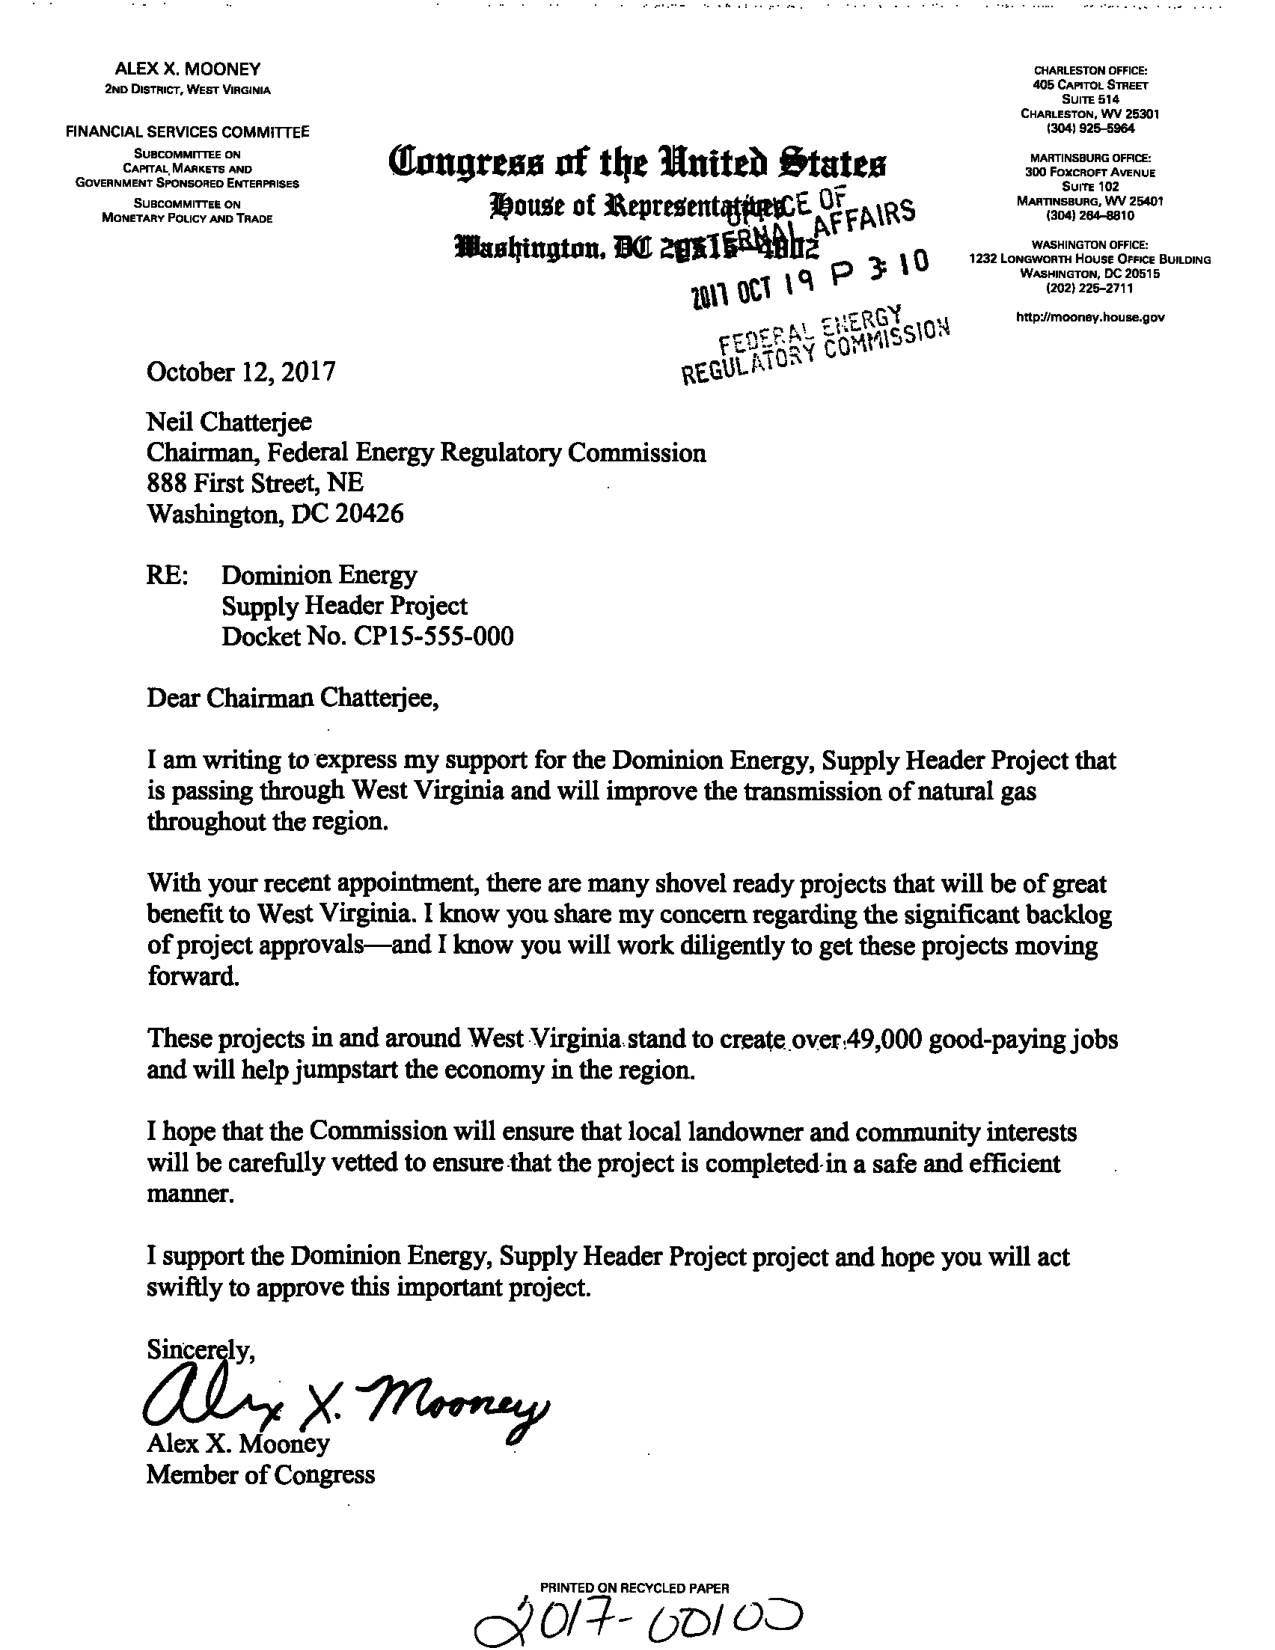
\includegraphics{20171020-0018-14718216}}
\end{center}
This is a letter written by Rep. Alex Mooney (R-WV2) to FERC on October 12, 2017. 

\end{frame}
%%%%%%%%%%%%%%%%%%%%%%%%%%%%%%
%%%%%%%%%%%%%%%%%%%%%%%%%%%%%%
\begin{frame} 
\frametitle{Example of Constituent Service Letter}
\begin{center}
\scalebox{0.3}{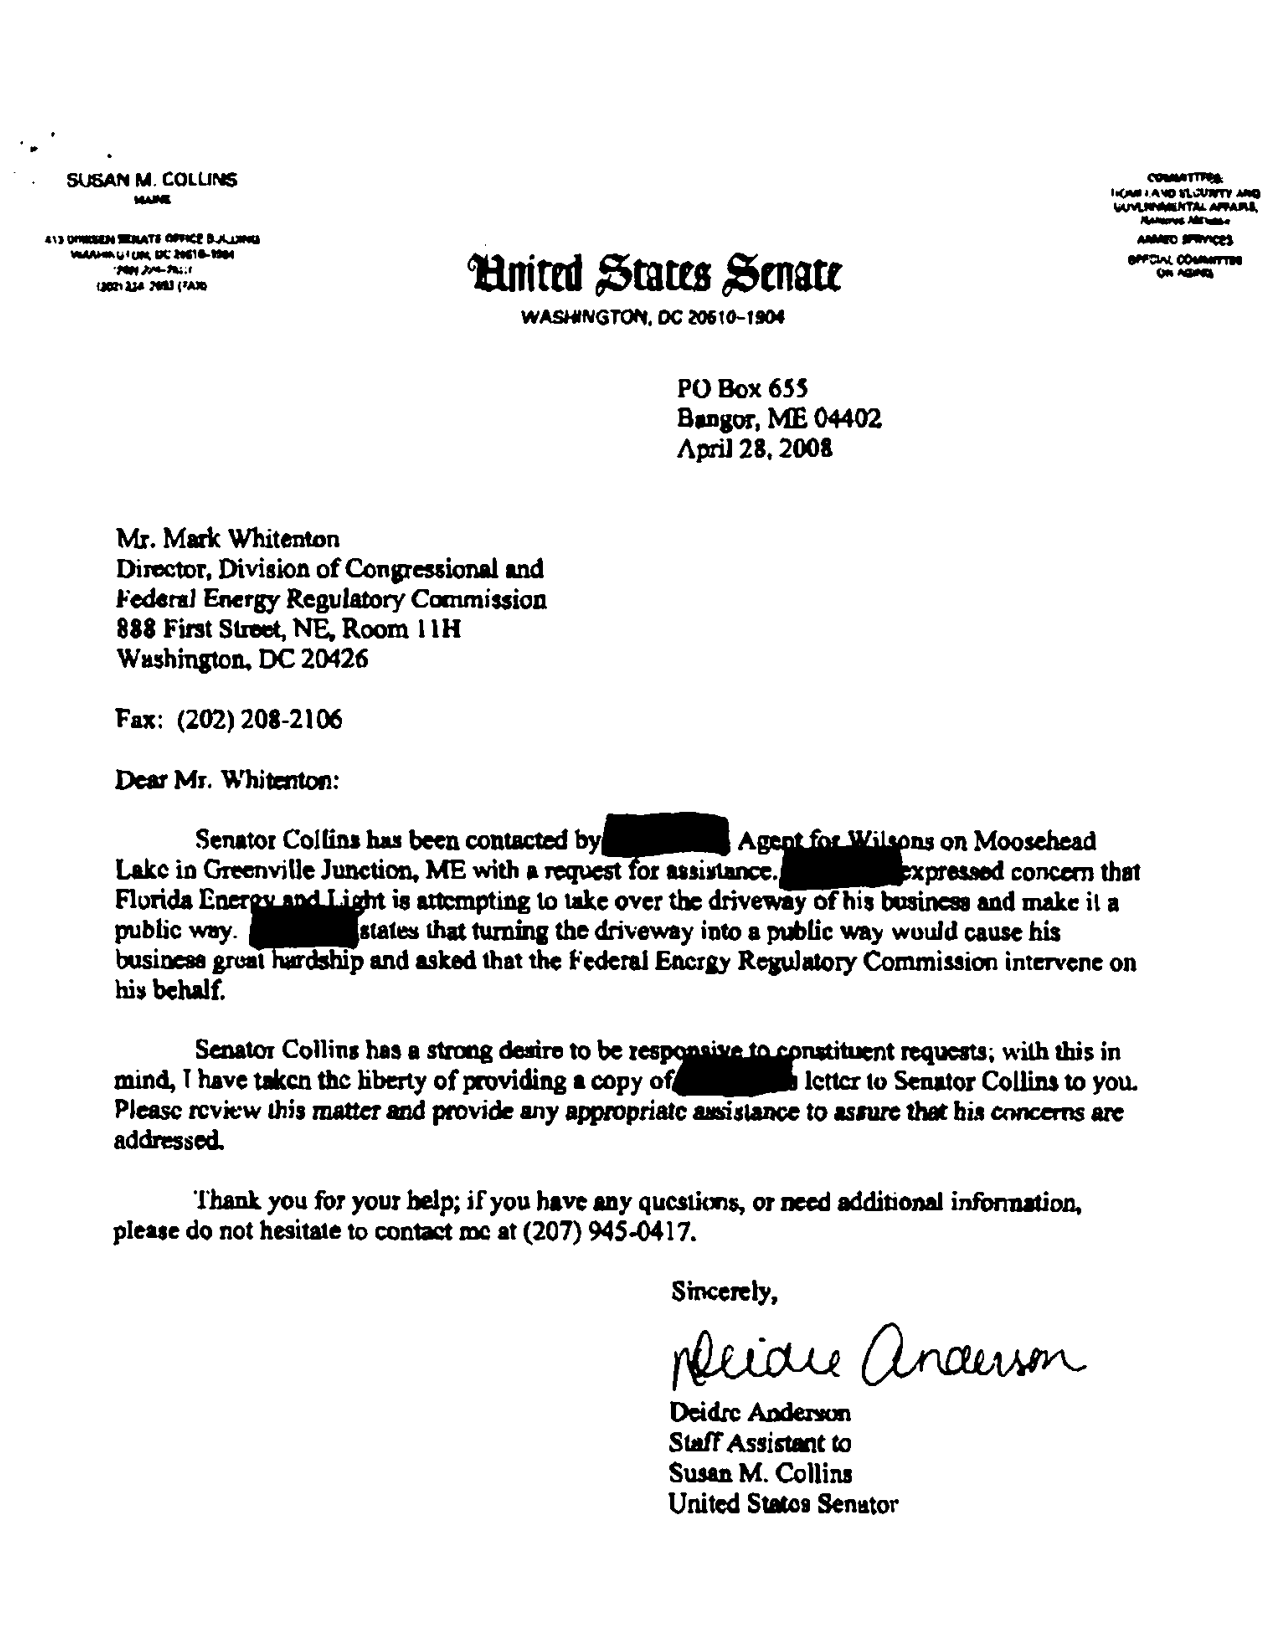
\includegraphics{20080515-0185small}}
\end{center}
This is a constituency service letter written by Senator Susan Collins (R-ME) to FERC on April 28, 2008.

\end{frame}
%%%%%%%%%%%%%%%%%%%%%%%%%%%%%%
\begin{frame}
\frametitle{FERC Data}
\Large
\begin{itemize}
\item Full text of all letters from Congress $\rightarrow$ FERC 
\bigskip
\item From January 1, 2000, and December 31, 2018
\bigskip
\item Every letter: human coder + automated processing
\bigskip
\item 6,988 members-level observations for 2000-2018
\item 4,780 member-level observations for 2000-2012 connected to campaign donations from the energy sector. 

\end{itemize}
\end{frame}
%%%%%%%%%%%%%%%%%%%%%%%%%%%%%%
\begin{frame} 
\frametitle{}
\Large
What Are Congressional Letters to FERC About?
\end{frame}
%%%%%%%%%%%%%%%%%%%%%%%%%%%%%%
%%%%%%%%%%%%%%%%%%%%%%%%%%%%%%
\begin{frame} 
\frametitle{The Distribution Across Types of Congressional Requests FERC vs. All* Agencies}

\centering
%\begin{subfigure}{\columnwidth}


\includegraphics[width=\textwidth]{data-by-type-1.png}
%\textbf{.} % x-axis shows our four categories of letters: 501c3 (i.e. non-profit) or local government, corporate constituent, individual constituent, and policy.  The y-axis shows the percentage of letters that were of that type.  The dark purple bars are for letters written to FERC (which is a subsidiary of the Department of Energy) and the mustard color bars are for the overall averages across all agencies that we have previously coded.  The numbers on top of each bar represent the total number of letters represented by the percentages.


\end{frame}
%%%%%%%%%%%%%%%%%%%%%%%%%%%%%%

\begin{frame} 
\frametitle{Studying the Influence of Campaign Contributions on Congressional-Bureaucratic Relations}
\Large
\begin{itemize}
\item Avenue for Influence: Letters to FERC less visible than roll call votes
\item High stakes for companies
\item Corporate PAC contributions from Energy Sector
\item Who Writes on Behalf of Constituents vs. Business?

\end{itemize}
\end{frame}
%%%%%%%%%%%%%%%%%%%%%%%%%%%%%%
%%%%%%%%%%%%%%%%%%%%%%%%%%%%%%
\begin{frame} 
\frametitle{}
\Large
\begin{center}
What Types of Letters are Supportive of Businesses?
\end{center}
\end{frame}
%%%%%%%%%%%%%%%%%%%%%%%%%%%%%%
%%%%%%%%%%%%%%%%%%%%%%%%%%%%%%
\begin{frame} 
\frametitle{What Types of Letters are Supportive of Businesses?}



\includegraphics[width=\textwidth]{constituent-non-constituent-1.png}
 %The left panel shows letters written to FERC on behalf of individual constituents and the right panel shows letters written to FERC on behalf of non-constituents.  The bars show what those letters were actually arguing for substantively broken down into four categories: against a named business (Antibusiness), in favor of a named business (Probusiness), both for and against named businesses (Both), and Other (other is a catch-all category that may include advocating for or against specific regulations which may benefit (or harm) a business, but no business names were mentioned in the letter. }


\end{frame}
%%%%%%%%%%%%%%%%%%%%%%%%%%%%%%
%%%%%%%%%%%%%%%%%%%%%%%%%%%%%%
\begin{frame} 
\Large
\begin{center}
What Members Attempt to Influence FERC?
\end{center}
\end{frame}
%%%%%%%%%%%%%%%%%%%%%%%%%%%%%%
%%%%%%%%%%%%%%%%%%%%%%%%%%%%%%
\begin{frame} 
\frametitle{Senators Writing the Most Letters to FERC}

\centering


%\caption{Senators Most Attempting to Influence FERC}\label{f:senatebarcode}

\includegraphics[width = \textwidth]{members_barcoded-1.png}
%\caption{Representatives Most Attempting to Influence FERC}\label{f:housebarcode}

%\textbf{Legislators Writing the Most Letters to FERC.} %The top panel shows the Senators who wrote the most letters to FERC and the bottom panel shows the Representatives who wrote the most letters to FERC.  Each hash mark indicates the legislator wrote a letter on that date. Note that many members listed in the table weren't in the chamber for the entire period, so blank stretches at the end or beginning of the line may indicate the member was out of office during that period.}


\end{frame}
%%%%%%%%%%%%%%%%%%%%%%%%%%%%%%
%%%%%%%%%%%%%%%%%%%%%%%%%%%%%%
\begin{frame} 
\frametitle{Representatives Writing the Most Letters to FERC}
\Large
\centering

\includegraphics[width = \textwidth]{members_barcoded-2.png}
\end{frame}
%%%%%%%%%%%%%%%%%%%%%%%%%%%%%%
%%%%%%%%%%%%%%%%%%%%%%%%%%%%%%
\begin{frame} 
\Large
\begin{center}
Who Writes on Behalf of Constituents vs. Business?

\pause 
\bigskip
\bigskip
By Party and Majority Status
\end{center}

\end{frame}
%%%%%%%%%%%%%%%%%%%%%%%%%%%%%%
%%%%%%%%%%%%%%%%%%%%%%%%%%%%%%
\begin{frame} 
\frametitle{Who Writes on Behalf of Constituents vs. Business?}
\centering


\includegraphics[width=\textwidth]{part-constituent-1.png}
\textbf{Figure \ref{f:party}: }. %The upper left panel represents of letters to FERC Democrats wrote while they were in the majority, what percentage were advocating on behalf of constituents and what percentage were advocating on behalf of businesses.  The upper right panel shows the same proportions for Republicans while they were in the majority, the lower right for Republicans while they were in the minority, and the lower left for Democrats while they were in the Minority. }



\end{frame}
%%%%%%%%%%%%%%%%%%%%%%%%%%%%%%
%%%%%%%%%%%%%%%%%%%%%%%%%%%%%%
\begin{frame} 
\Large
\begin{center}
Demand Driven Letter-writing?
\end{center}
\end{frame}
%%%%%%%%%%%%%%%%%%%%%%%%%%%%%%
%%%%%%%%%%%%%%%%%%%%%%%%%%%%%%
\begin{frame} 
\frametitle{State population and Senate Letter-writing}
\Large

\centering


\includegraphics[width=\linewidth]{population-1.png}
\end{frame}
%%%%%%%%%%%%%%%%%%%%%%%%%%%%%%
%%%%%%%%%%%%%%%%%%%%%%%%%%%%%%
\begin{frame} 
\frametitle{FERC Contacts from Senators by State}
\Large
\centering

\includegraphics[width=\linewidth]{sentate_percapita_map-2.png}

%\caption*{\textbf{Figure \ref{f:statepoptotal}: FERC Contacts from Senators by State.} The left panel shows the total number of FERC contacts from senators by state.  The right panel shows the contact per million residents from senators by state. Lighter colors show greater letter-writing activity.}
%\end{figure}
%\end{center}
\end{frame}
%%%%%%%%%%%%%%%%%%%%%%%%%%%%%%
%%%%%%%%%%%%%%%%%%%%%%%%%%%%%%
\begin{frame} 
\frametitle{}
\Large
\begin{center}
Committee Chairs Attempting to Influence FERC?
\end{center}
\end{frame}
%%%%%%%%%%%%%%%%%%%%%%%%%%%%%%
%%%%%%%%%%%%%%%%%%%%%%%%%%%%%%
\begin{frame} 
\frametitle{Committee Chairs Attempting to Influence FERC}

\centering

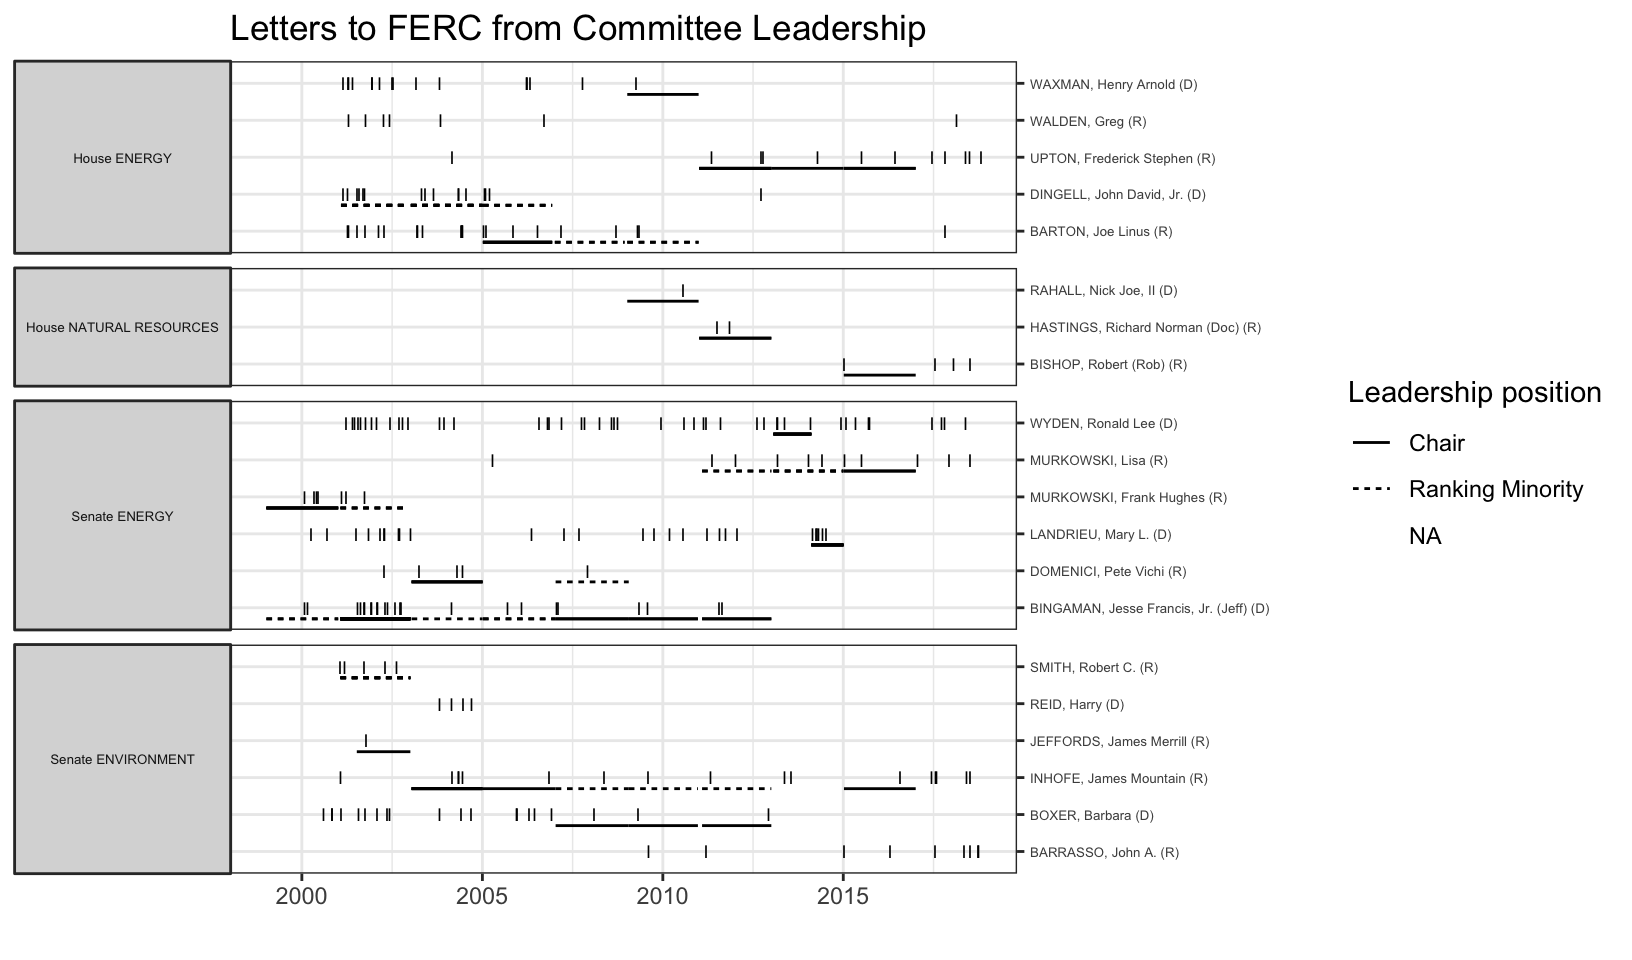
\includegraphics[width = \textwidth]{committeechiars_barcode-1.png}
%\caption*{\textbf{Figure \ref{f:chairs}: Committee Chairs Attempting to Influence FERC.} Each hash mark indicates the legislator wrote a letter on that date. The solid horizontal lines indicate the period for which that member was a committee chair; the dashed horizontal lines indicate the period for which that member was ranking member (top minority party leader) of the committee.  Note that many members listed in the table weren't in the chamber for the entire period, so blank stretches at the end or beginning of the line may indicate the member was out of office during that period.}

\end{frame}
%%%%%%%%%%%%%%%%%%%%%%%%%%%%%%
%%%%%%%%%%%%%%%%%%%%%%%%%%%%%%
\begin{frame} 
\frametitle{}
\Large
\begin{center}
Exploring the Relationship between Letter-writing and Campaign Contributions
\end{center}
\end{frame}
%%%%%%%%%%%%%%%%%%%%%%%%%%%%%%
%%%%%%%%%%%%%%%%%%%%%%%%%%%%%%
\begin{frame} 
\frametitle{Measuring Industry Money}
\Large
\begin{itemize}
\item Campaign contribution data from Adam Bonica's Database on Ideology, Money in Politics, and Elections 
\ bigskip
\item Center for Responsive Politics' industry classification of PACs.
\end{itemize}
\end{frame}
%%%%%%%%%%%%%%%%%%%%%%%%%%%%%%
%%%%%%%%%%%%%%%%%%%%%%%%%%%%%%
\begin{frame} 
\frametitle{Average Energy Sector PAC Contributions Per Member Per Cycle}

\centering

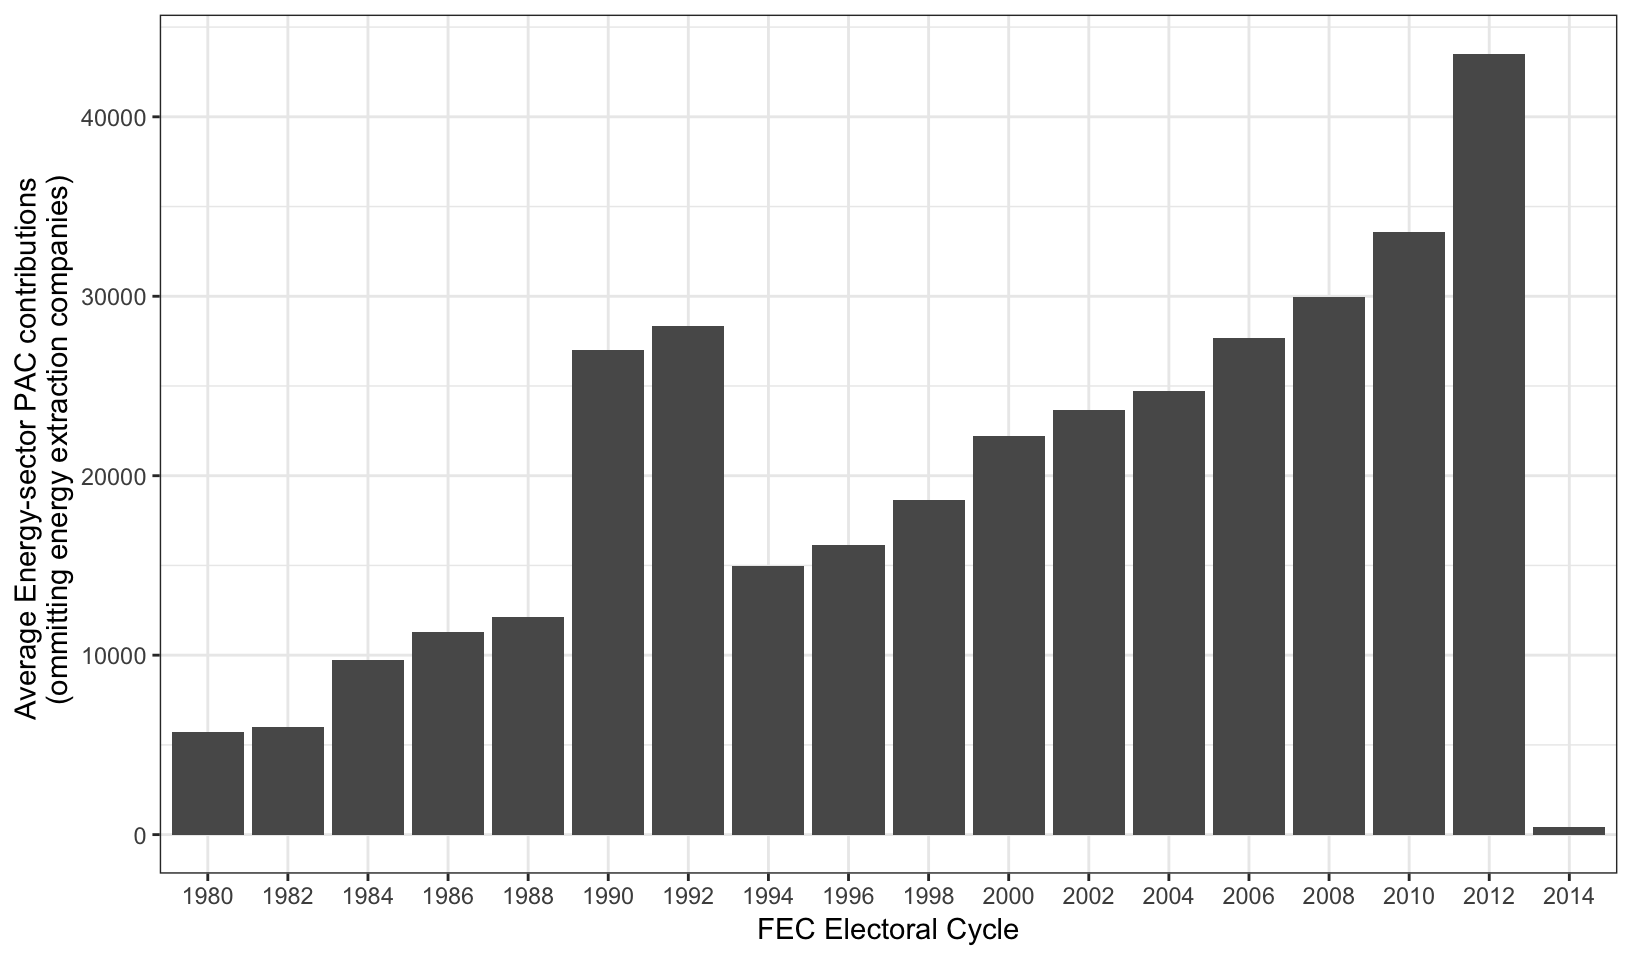
\includegraphics[width = \textwidth]{letters_PACs-data-1.png}

\end{frame}
%%%%%%%%%%%%%%%%%%%%%%%%%%%%%%
%%%%%%%%%%%%%%%%%%%%%%%%%%%%%%
\begin{frame} 
\frametitle{Partisan Differences in Energy \$}

\centering
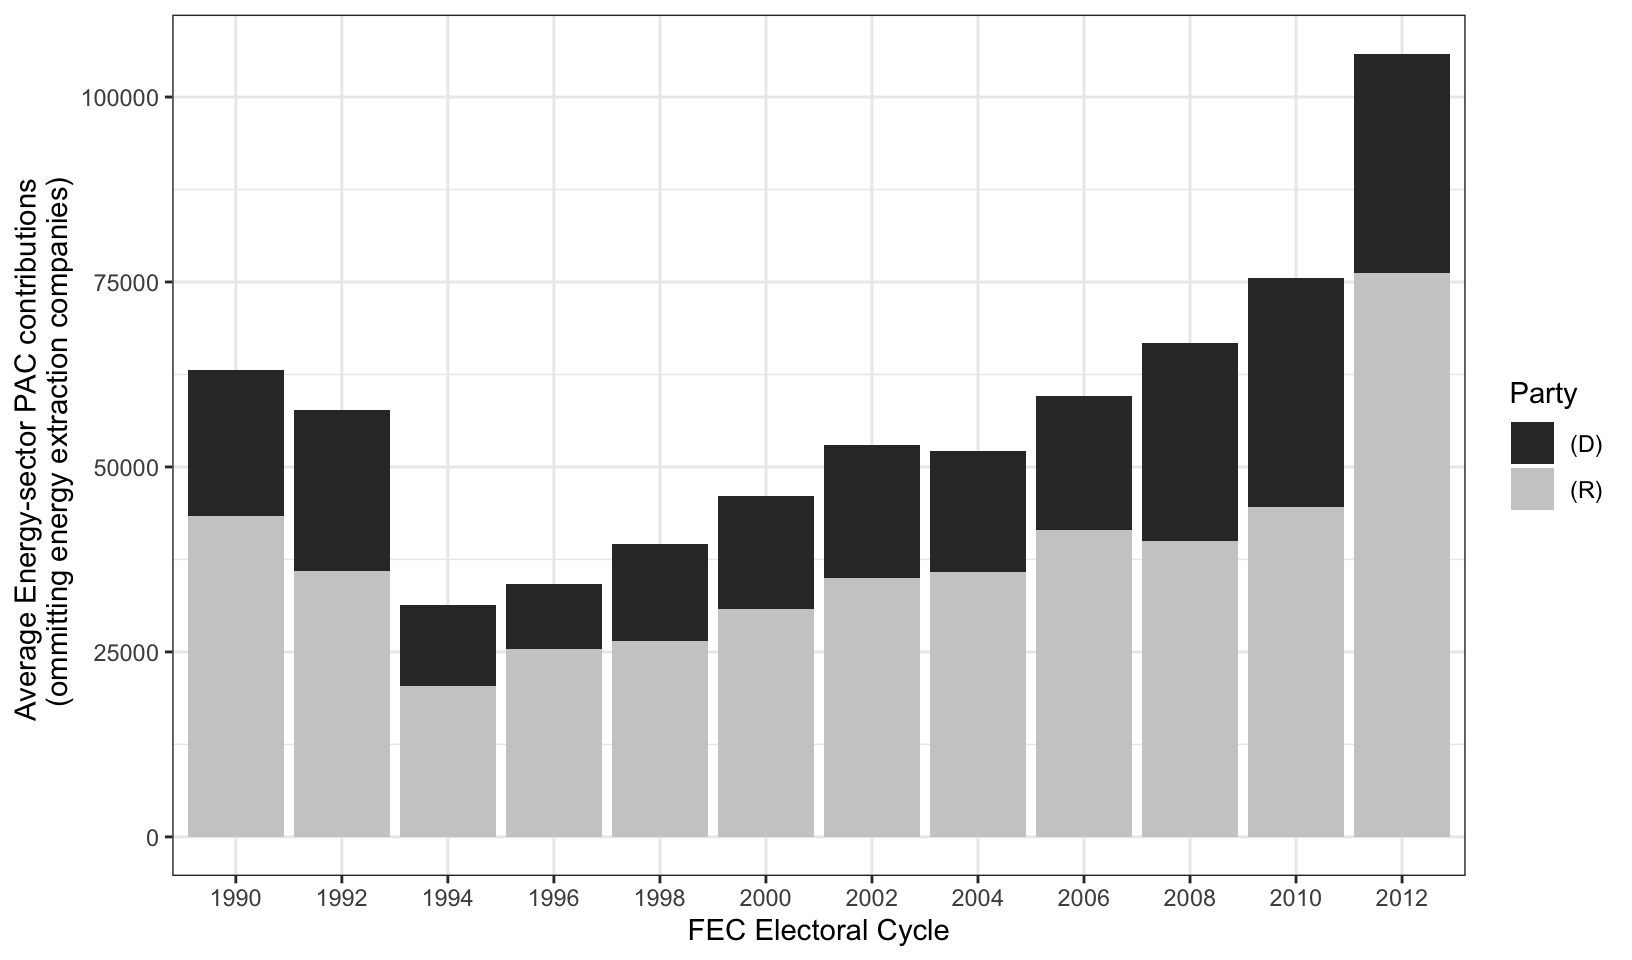
\includegraphics[width = \textwidth]{letters_money-2.png}

\end{frame}
%%%%%%%%%%%%%%%%%%%%%%%%%%%%%%
%%%%%%%%%%%%%%%%%%%%%%%%%%%%%%
\begin{frame} 

\Large
\begin{center}
Preliminary Results: Relationship between Letter-writing and Campaign Contributions?
\end{center}
\end{frame}
%%%%%%%%%%%%%%%%%%%%%%%%%%%%%%
%%%%%%%%%%%%%%%%%%%%%%%%%%%%%%
\begin{frame} 
\frametitle{Campaign Contributions and Letter-writing to FERC}

\centering

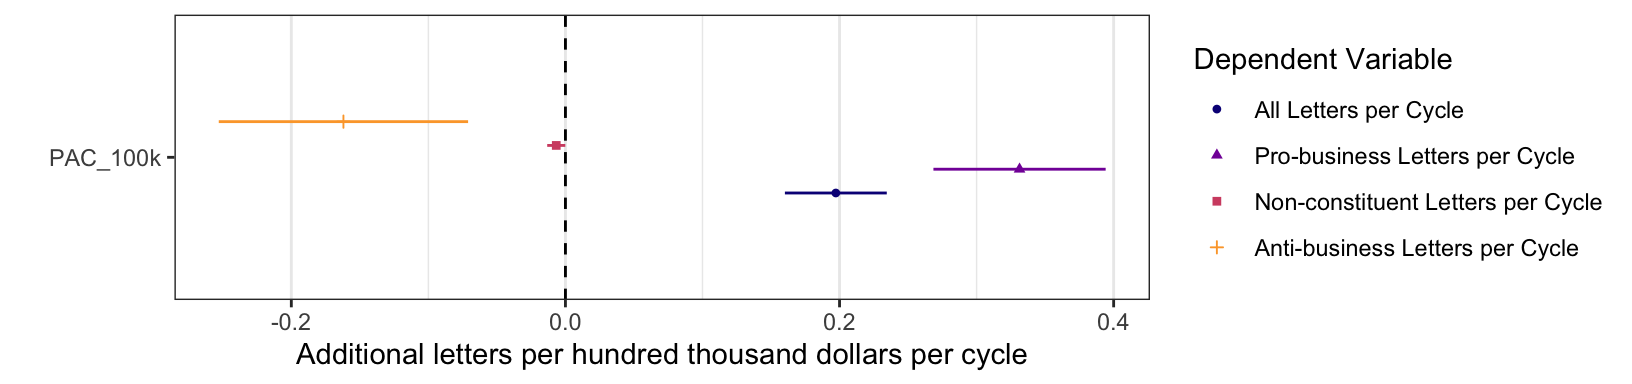
\includegraphics[width = \textwidth]{models-1.png}

\end{frame}
%%%%%%%%%%%%%%%%%%%%%%%%%%%%%%
%%%%%%%%%%%%%%%%%%%%%%%%%%%%%%
\begin{frame} 
\frametitle{Campaign Contributions, Party and Letter-writing to FERC}
\Large

\centering

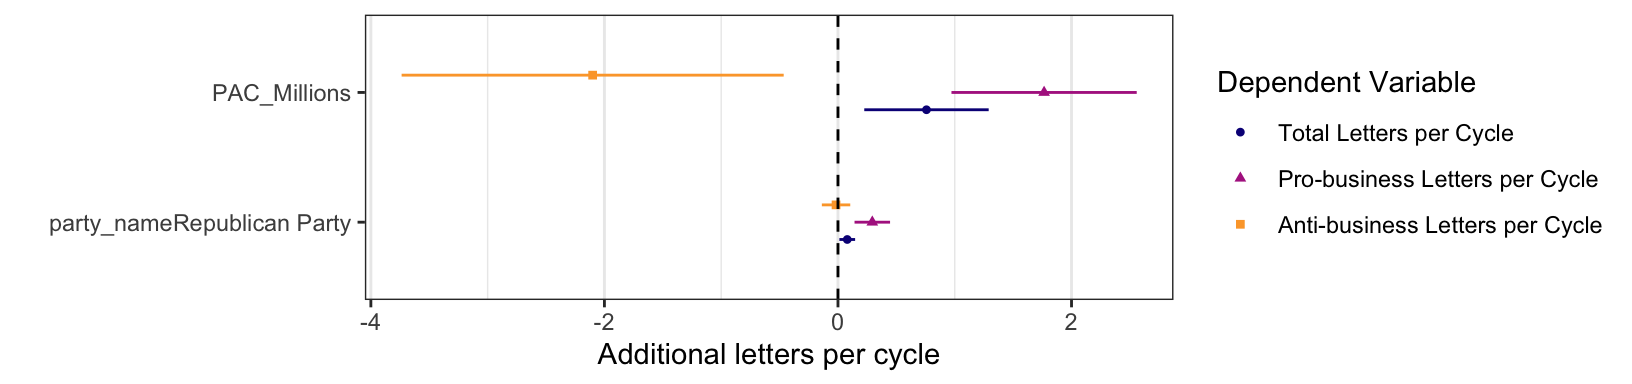
\includegraphics[width = \textwidth]{models-full-1.png}

\end{frame}
%%%%%%%%%%%%%%%%%%%%%%%%%%%%%%


%%%%%%%%%%%%%%%%%%%%%%%%%%%%%%
\begin{frame} 
\frametitle{Next Steps}
\Large
\begin{itemize}
\item Connecting Companies in Letters to Campaign Contributions
\begin{itemize}
\item Challenge: Linking Energy Projects, Subsidiary Companies and Parent Companies
\end{itemize}
\bigskip
\item Impact of Letters on Outcomes
\begin{itemize}
\item Speed of FERC Review
\end{itemize}
\end{itemize}
\end{frame}
%%%%%%%%%%%%%%%%%%%%%%%%%%%%%%
%%%%%%%%%%%%%%%%%%%%%%%%%%%%%%
\begin{frame} 
\frametitle{Conclusions}
\Large
\begin{itemize}
\item New Window into Congressional-Bureaucracy: Congressional Letters
\item Extensive advocacy on behalf of businesses
\item We find that Republicans and those who receive money from the energy-sector write relatively more letters on behalf of energy companies, but not on behalf of constituents
\item Democrats write comparatively more letters in opposition to energy companies
\end{itemize}
\end{frame}
%%%%%%%%%%%%%%%%%%%%%%%%%%%%%%
%%%%%%%%%%%%%%%%%%%%%%%%%%%%%%
\begin{frame}
\centering
\huge
Thank you! 
\end{frame}
%%%%%%%%%%%%%%%%%%%%%%%%%%%%%%%%
\appendix
\begin{frame}
\maketitle
\end{frame}

\begin{frame}
\frametitle{Correspondence Data}
Environmental Protection Agency
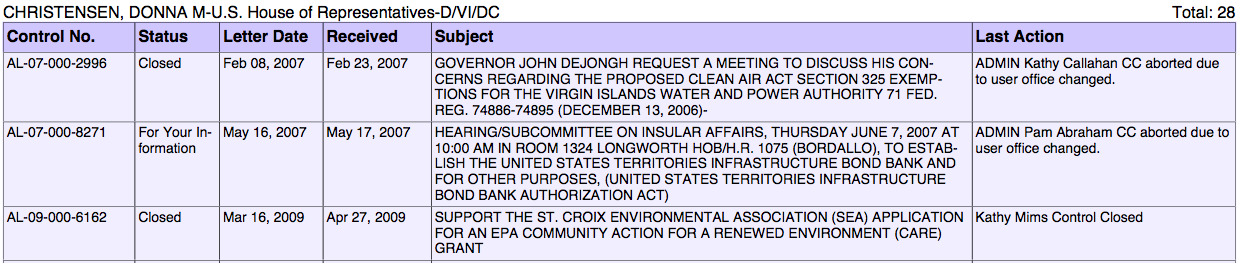
\includegraphics[width = \textwidth]{EPA}
% rich and informative summaries like those kept by the EPA. Here, Rep Donna writes about a regulatory exemption for a power plant, to alert EPA to a hearing, and in support of a nonprofit grant application.
\end{frame}


% To give you a sense of the range of responses. Some agencies provided letters themselves,

%{SLIDE}

% others provided logs, which range widely in the amount of information they record. 
% from, at the worst, handwritten logs with obscure acronyms to indicate the topic, as in this log from ICE
\begin{frame}
\frametitle{Correspondence Data}
Department of Homeland Security Immigration and Customs Enforcement (ICE)
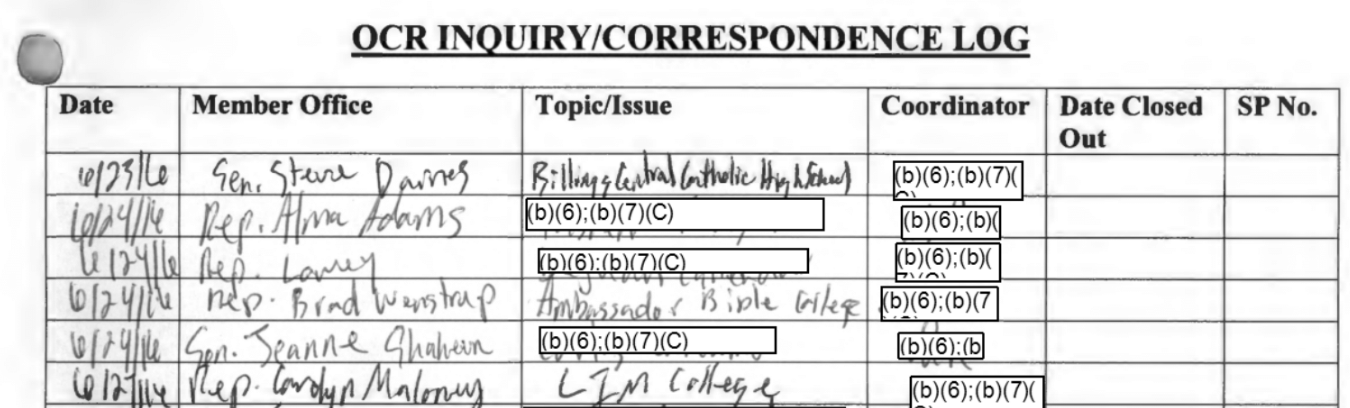
\includegraphics[width = \textwidth]{ICE}
\end{frame}

% Or, in contrast [SLIDE]
\begin{frame}
\frametitle{Correspondence Data}
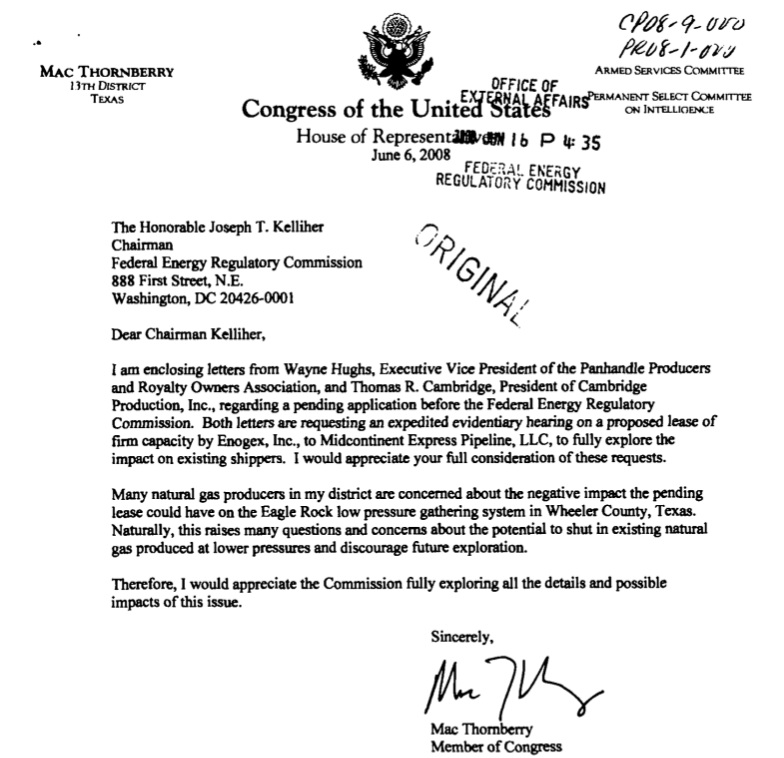
\includegraphics[width = \textwidth]{FERC}
% For example, here Rep. Thornberry, chair of armed services committee is writing to Federal Energy Regulatory Commission on behalf of two companies in his district, asking for extra scrutiny on a another company's permit application. 

% We have several thousand such letters written to this agency, which we use optical content recognition to extract the text. If they do not have metadata like the sender's name and date, we extract it from the text of the letter or discription of the letter.
\end{frame}


%^%%%%%%%%%%%
\begin{frame}
\frametitle{Agency Character: CIA $\#$OnBrand}
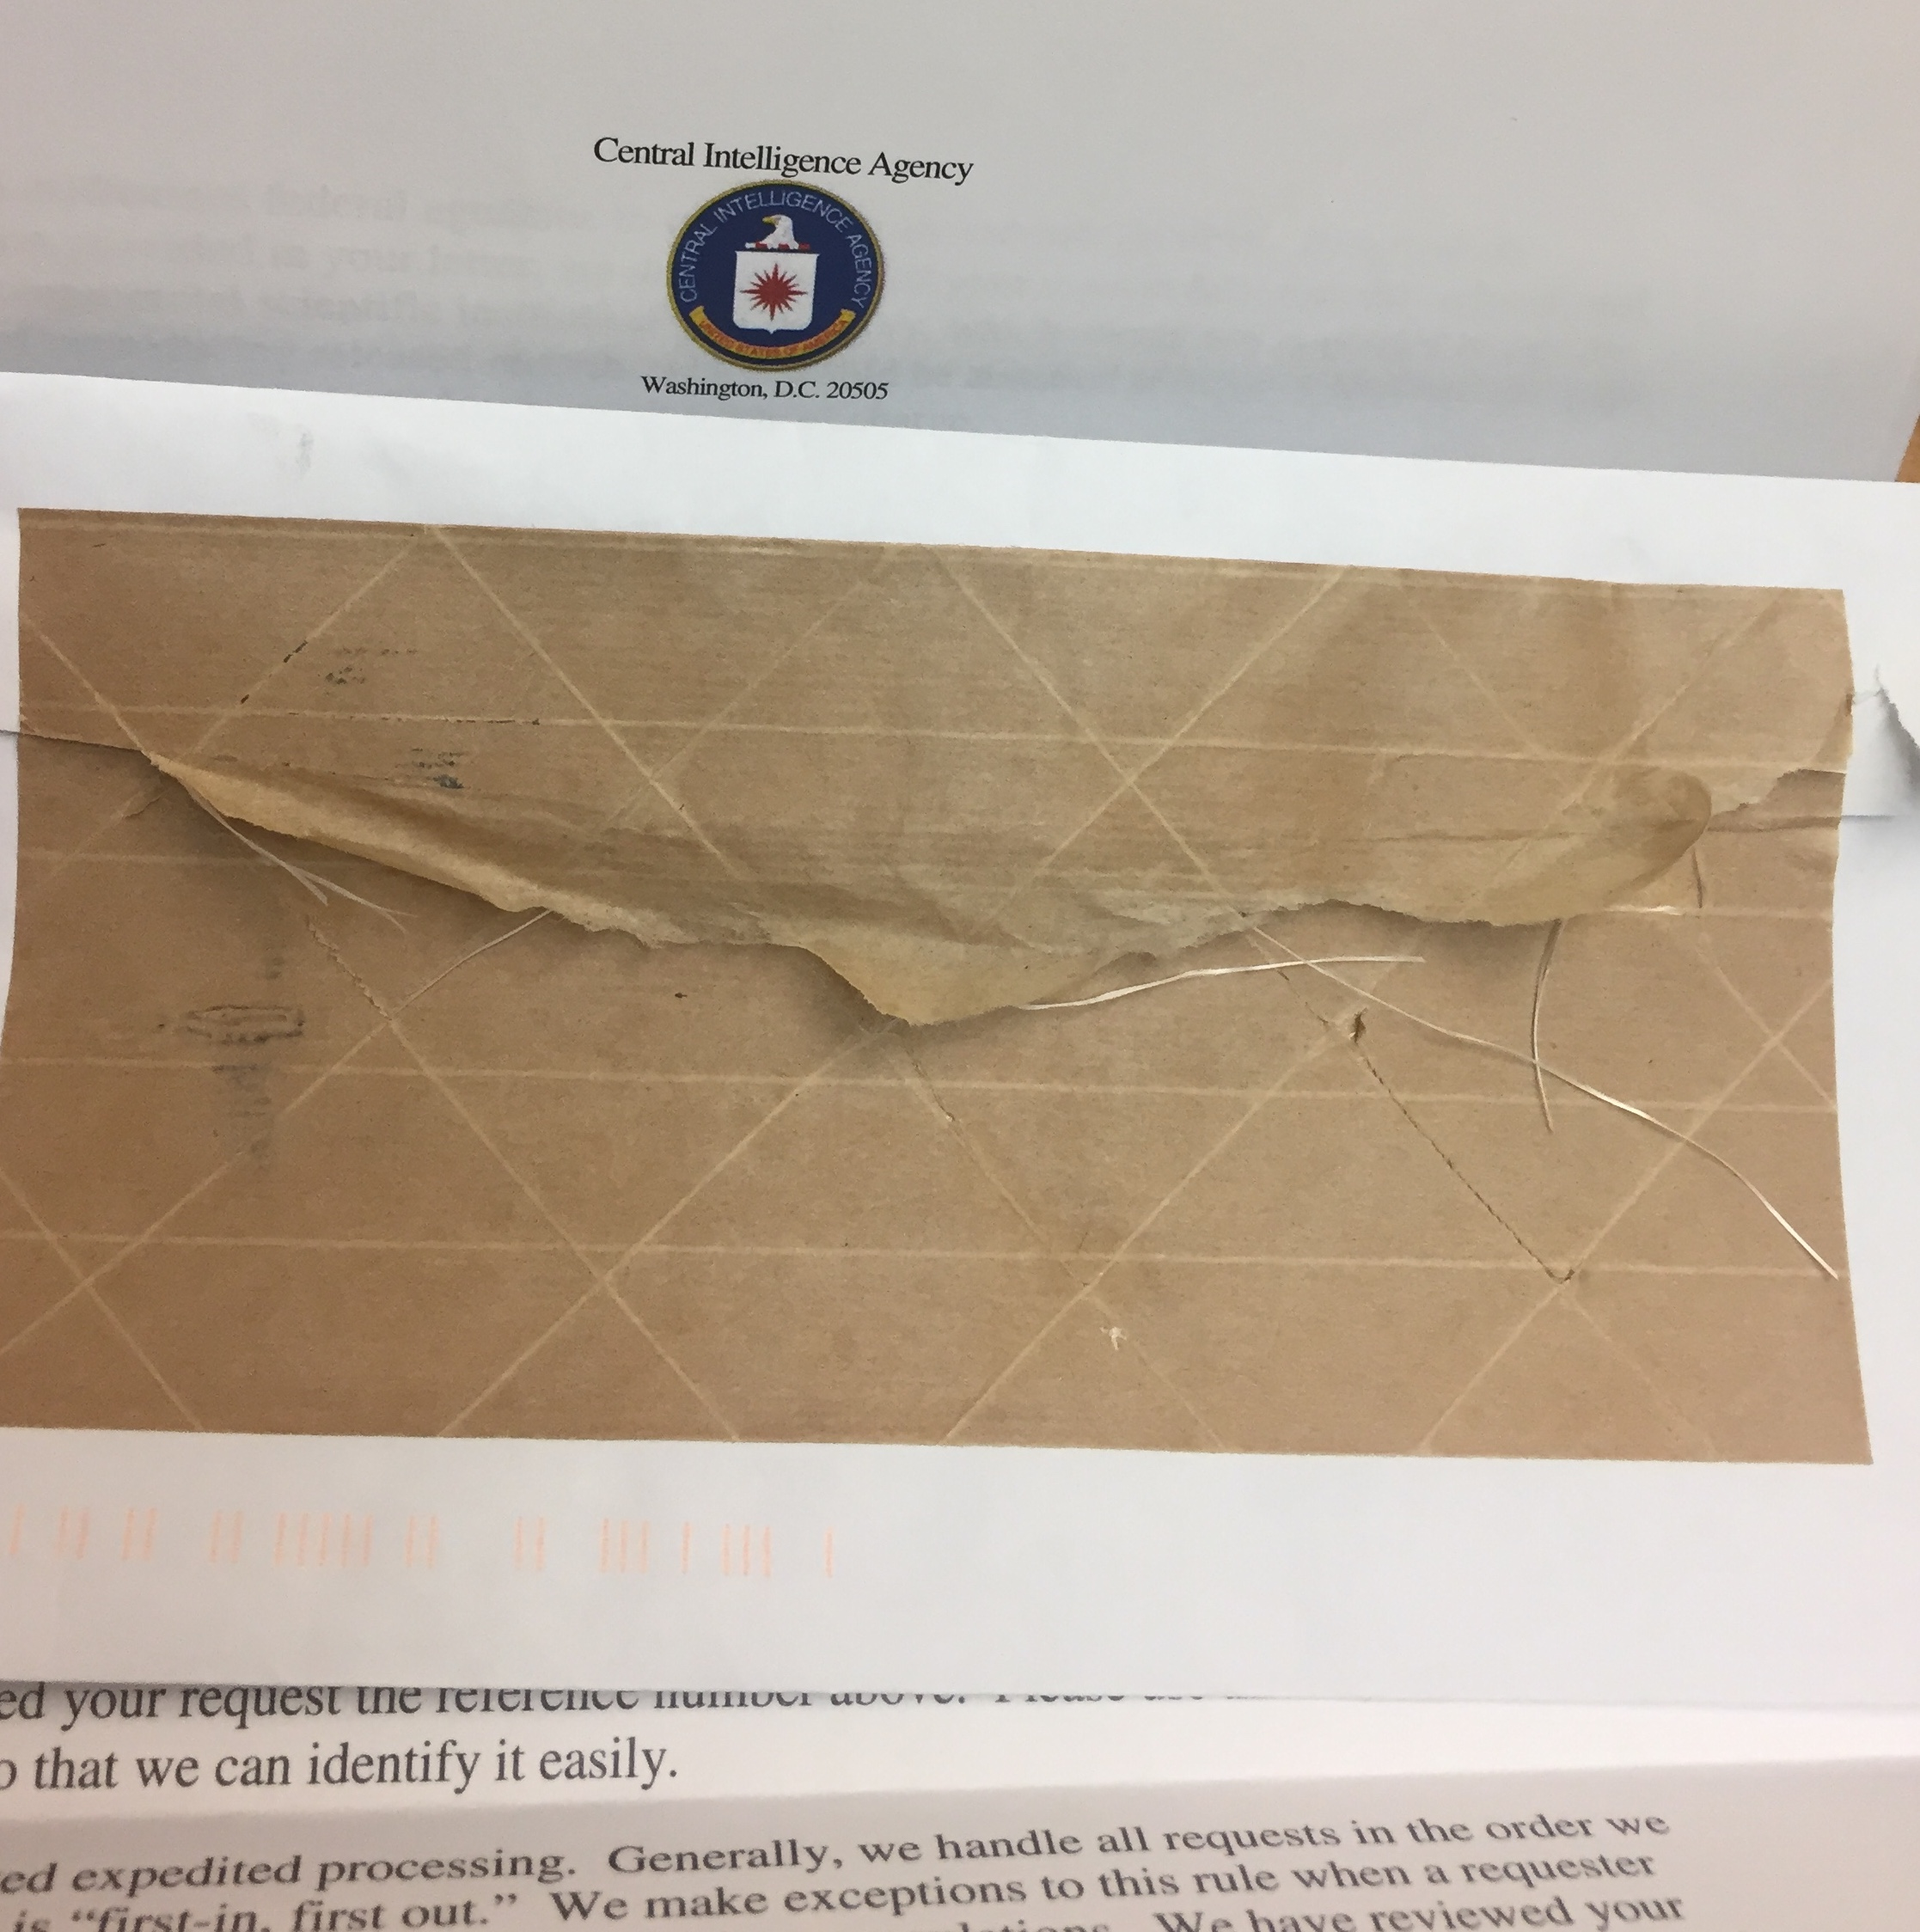
\includegraphics[width = \textwidth]{CIACorrespondence}
\end{frame}
%%%%%%%%%%%%%%%%%%%%%%%
\begin{frame}
\centering
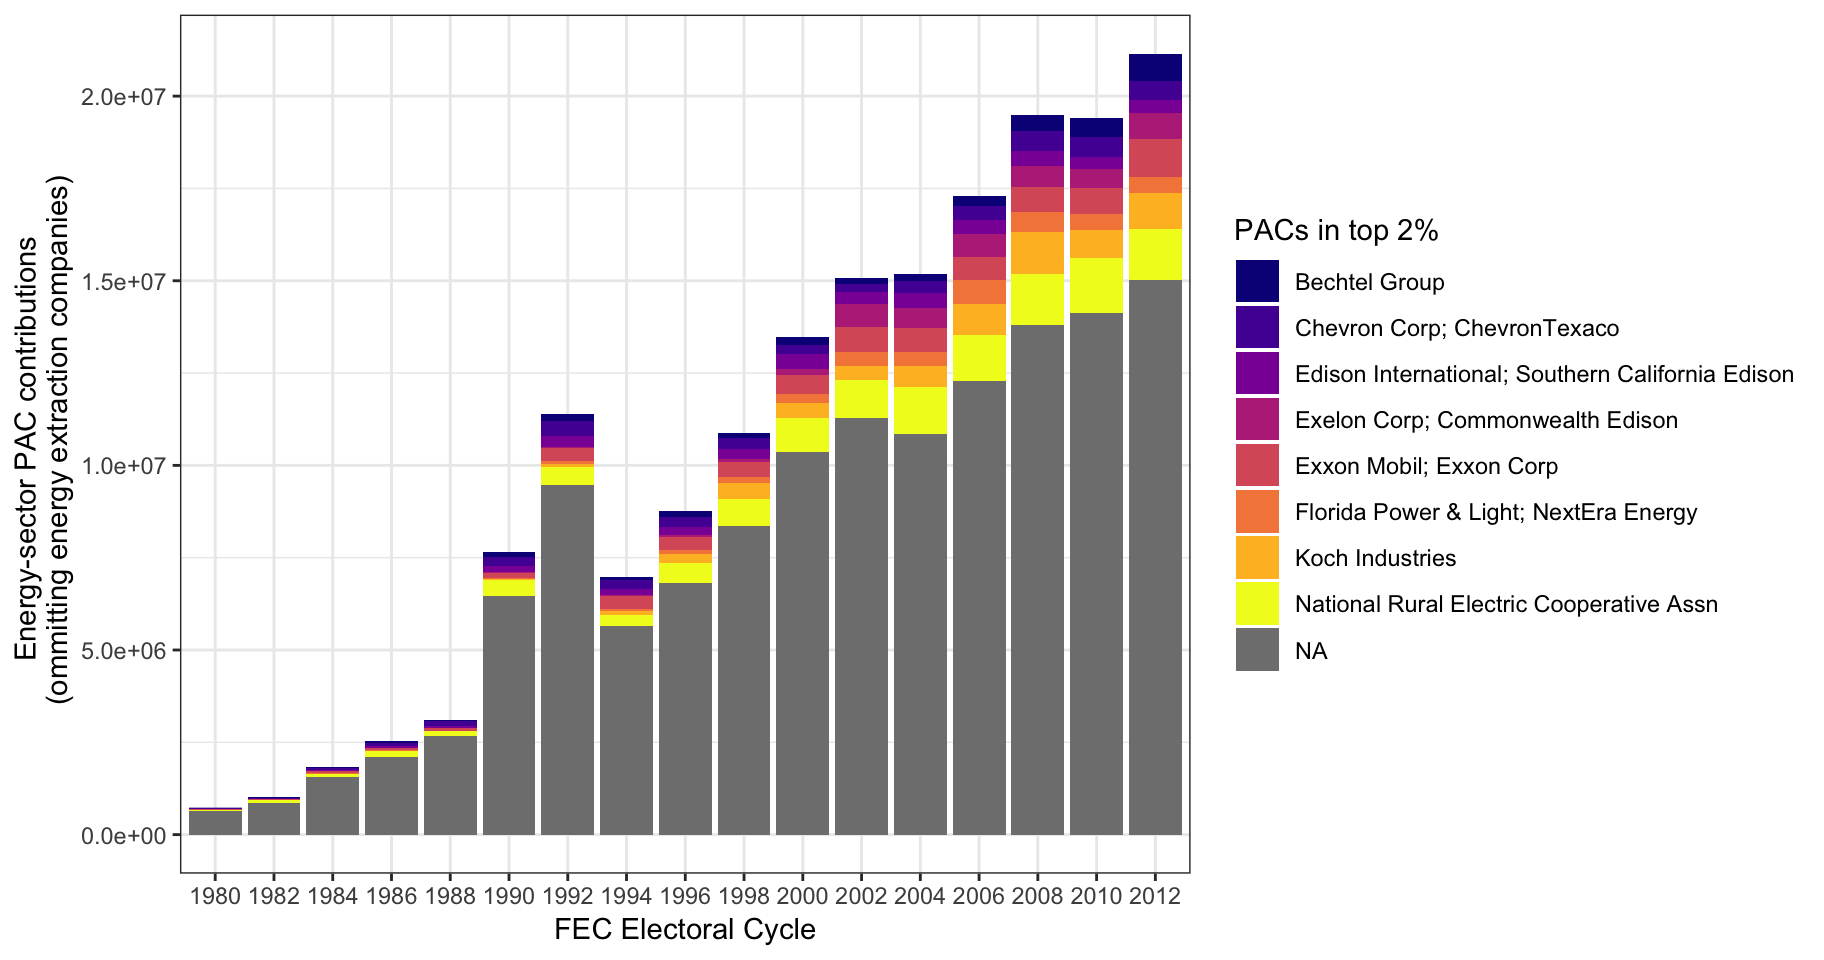
\includegraphics[width = \textwidth]{letters_PACs-data-2.png}
\textbf{ Unequal Money Across Energy Sector PACs}
\end{frame} 
%%%%%%%%%%%%%%%%%%%%%%%
%%%%%%%%%%%%%%%%%%%%%%%%%%%%%%%%

\begin{frame}
\frametitle{Our Correspondence Data}
\scriptsize
% response table
\begin{table}[!htbp] \centering 
  % \caption{} 
  \label{} 
\begin{tabular}{@{\extracolsep{5pt}} lcccc} 
 & FOIAed  & Records & Coded & N \\ 
 &Components&Received&&\\
\hline \\[-1.8ex] 
Department of Agriculture & 29 & 29 & 11 & 1957 \\ 
Department of Commerce & 18 & 18 & 10 & 6875 \\ 
Department of Defense & 49 & 10 & 7 & 5479 \\ 
Department of Education & 1 & 1 & 1 & 3868 \\ 
Department of Energy & 8 & 2 & 1 & 1269 \\ 
Department of Health and Human Services & 15 & 7 & 5 & 6199 \\ 
Department of Homeland Security & 6 & 5 & 5 & 26435 \\ 
Department of Housing \& Urban Dev. & 2 & 0 & 0 & 0 \\ 
Department of Justice & 11 & 1 & 1 & 903 \\ 
Department of Labor & 24 & 9 & 6 & 22936 \\ 
Department of State & 1 & 0 & 0 & 0 \\ 
Department of the Interior & 10 & 6 & 5 & 5171 \\ 
Department of the Treasury & 8 & 5 & 4 & 11143 \\ 
Department of Transportation & 10 & 6 & 6 & 18482 \\ 
Department of Veterans Affairs & 3 & 0 & 0 & 0 \\ 
\hline \\[-1.8ex] 
Independent Agencies & 38 & 21 & 18 & 46182 \\ 
\hline \\[-1.8ex] 
Total & 233 & 120 & 80 & 156899 \\ 
\hline \\[-1.8ex] 
\end{tabular} 
\end{table} 

\end{frame}





\end{document}